% Nallino, Part II p. 246, second figure: the true arc of retrogradation, redrawn from the print at the size of the
% print. The coordinates are those of a 400 dpi render of the figure (crop from x 402 pt, y 370 pt of the master
% page; y downward). The epicycle has its centre in H; QHE' goes to the centre of the equant, PHDE to the Earth E,
% TE from the planet T; the dashed line hdE is the line of the true perigee d when the centre has moved to h.
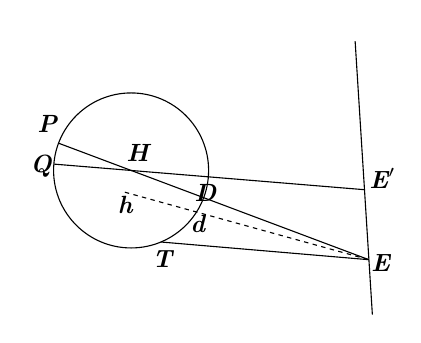
\begin{tikzpicture}[x=0.0635mm,y=-0.0635mm,line width=0.4pt,every node/.style={font=\bfseries\itshape\small,inner sep=1pt}]
\path (37,21);
\coordinate (H) at (229.5,306.5);
\coordinate (Ep) at (696,345);
\coordinate (E) at (705,485);
\coordinate (Q) at (75,293.8);
\coordinate (P) at (84.4,252);
\coordinate (T) at (289,449.6);
\coordinate (h) at (217,350);
\draw (H) circle[radius=155];
\draw (677.5,48) -- (712,595);
\draw (Q) -- (Ep);
\draw (P) -- (E);
\draw (T) -- (E);
\draw[dash pattern=on 1.6pt off 1.6pt] (h) -- (E);
\node at (61.5,214) {P};
\node at (49.5,298) {Q};
\node at (242.5,271) {H};
\node at (218,375.5) {h};
\node at (378,352) {D};
\node at (363,414) {d};
\node at (292,484) {T};
\node at (725,322) {E\rlap{$'$}};
\node at (728.5,491.5) {E};
\end{tikzpicture}
